\documentclass{beamer}
\usepackage[french]{babel}
\usepackage{hyperref}
\definecolor{links}{HTML}{2A1B81}
\hypersetup{colorlinks,linkcolor=,urlcolor=links}
\usepackage{graphicx}
\usepackage{amsmath,amssymb}
\usepackage{tabularx}
\usepackage{booktabs}
\usepackage[compatibility=false]{caption}
\usepackage[toc,page]{appendix}
\usepackage{minted}
\usepackage{xspace}

\makeatletter
  \def\beamer@calltheme#1#2#3{%
    \def\beamer@themelist{#2}
    \@for\beamer@themename:=\beamer@themelist\do
    {\usepackage[{#1}]{\beamer@themelocation/#3\beamer@themename}}}

  \def\usefolder#1{
    \def\beamer@themelocation{#1}
  }
  \def\beamer@themelocation{}

\patchcmd{\minted@colorbg}{\noindent}{\medskip\noindent}{}{}
\apptocmd{\endminted@colorbg}{\par\medskip}{}{}
\makeatother

\newcolumntype{Y}{>{\centering\arraybackslash}X}

\usefolder{../theme}
\usetheme[numbering=fraction,block=fill,progressbar=frametitle]{metropolis} %Use metropolis theme

\definecolor{bg}{rgb}{0.95,0.95,0.95}
\setminted{bgcolor=bg,fontsize=\scriptsize,autogobble,mathescape,breaklines,tabsize=2}
\setmintedinline{breaklines,autogobble,fontsize=\scriptsize}
\setbeamersize{text margin left=8pt,text margin right=8pt}
\setbeamercovered{transparent}

\begin{document}

\title[C++]{Introduction à la programmation en C++}
\author[nicolas.audebert@onera.fr]{Nicolas Audebert}
\setmainfont{Fira Sans}


\AtBeginSection[]{
  \begin{frame}{Plan de la séance}
  \small \tableofcontents[currentsection]
  \end{frame}
}

\newcommand\cppi[1]{\mintinline{cpp}{#1}}
\newcommand\cpp[1]{%
  \begin{minted}{cpp}
  #1
  \end{minted}
}%

\subtitle{Variables, structures conditionnelles, boucles et fonctions}
\date{21 septembre 2018}
\maketitle

\section{Rappels}
\begin{frame}{Dans l'épisode précédent\dots}

\begin{block}{Les langages de programmation}
Les langages de programmation comportent une syntaxe et une grammaire permettant d'exprimer des instructions humainement compréhensibles, qui seront traduites pour être exécutées par la machine. Dans ce cours, nous étudierons le \textbf{C++}.
\end{block}

\begin{exampleblock}{Compilation ou interprétation}
C++ est un langage \textbf{compilé} : la traduction C++ $\rightarrow$ langage machine est réalisée par le \textbf{compilateur} avant l'exécution. L'exécutable généré peut être utilisé n'importe où.

Python est un langage \textbf{interprété} : la traduction Python $\rightarrow$ langage machine est réalisée à la volée par l'\textbf{interpréteur}, qui est nécessaire pour exécuter le programme.
\end{exampleblock}

\end{frame}

\section{C++}

\begin{frame}{Une brève histoire du C++}

\begin{minipage}{0.33\textwidth}
  \centering
  
  
\includegraphics[width=0.7\textwidth]{images/cpp.png}
  
  {\footnotesize Logo du langage C++}
  \medskip
  
  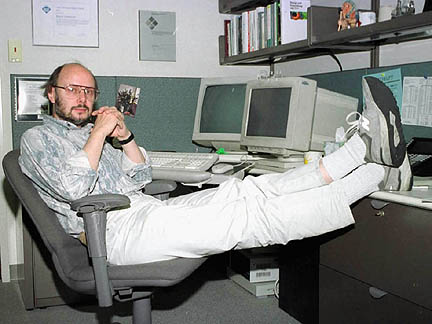
\includegraphics[width=0.9\textwidth]{images/bjarne.jpg}
  
  {\footnotesize Bjarne Stroustrup, créateur du C++ (\href{https://fr.wikipedia.org/wiki/Bjarne_Stroustrup}{Wikipédia})}
\end{minipage}%
\begin{minipage}{0.65\textwidth}
\begin{block}{Historique du C++}
  \begin{itemize}
    \item 1983 : débuts du C++, premier compilateur
    \item 1985 : \emph{The C++ Programming Language}, premier manuel de référence
    \item 1989 : version 2.0 du langage
    \item 1998 : première standardisation du langage
    \item 2003, 2011, 2014, 2017 : mises à jour du langage (actualisation du standard, nouvelles fonctionnalités)
    \item 2020 : prochaine standardisation 
  \end{itemize}
\end{block}
\end{minipage}
\end{frame}

\begin{frame}{Pourquoi le C++ ?}

\begin{block}{C et C++}
C++ est une augmentation du langage C pour lui en fournir de nouvelles fonctionnalités :
\begin{itemize}
  \item Les classes (et la notion d'objets),
  \item La gestion des exceptions,
  \item La surcharge des opérateurs,
  \item Les templates,
  \item Les espaces de noms,
  \item \dots
\end{itemize}
\end{block}

C++ comporte également une bibliothèque standard riche.

C++ est un langage \textbf{libre de droit}.
\end{frame}

\section{Variables}

\begin{frame}[fragile]
	\frametitle{Type des variables}
	\begin{block}{Langage typé}
  Dans un \textbf{langage typé}, les variables représentent une catégorie fixée d'objets et ne peuvent en changer. C++ est un langage typé.
	\end{block}
	\vfill
	\begin{minipage}{0.38\linewidth}
\uncover<1>{\mintinline{cpp}{1: int i;}}\\
\uncover<2>{\mintinline{cpp}{2: i = 2;}}\\
\uncover<3>{\mintinline{cpp}{3: float d = 5.6;}}\\
\uncover<4>{\mintinline{cpp}{4: char a = 'z';}}\\
\uncover<5>{\mintinline{cpp}{5: bool v = true;}}
	\end{minipage}
	\hfill
	\begin{minipage}{0.58\linewidth}
		\begin{enumerate}
			\item<1> Déclaration d'un entier \texttt{\textbf{i}}
      \item<2> Affectation de la valeur 2 à \texttt{\textbf{i}}
			\item<3> Déclaration et affectation d'un réel \texttt{\textbf{d}}
      \item<4> Idem pour un caractère \texttt{\textbf{a}}
      \item<5> Idem pour un booléen \texttt{\textbf{v}}
		\end{enumerate}
	\end{minipage}
\end{frame}

\begin{frame}[fragile]
	\frametitle{Déclaration et affectation d'une variable}
	\begin{block}{Déclaration}
		La déclaration annonce l'existence d'une variable:\\
		\centering
		\texttt{\textbf{type} nom\_de\_variable \textbf{\huge ;}}
	\end{block}
	\begin{block}{Affectation}
	  L'affectation assigne une valeur à une variable déclarée:\\
		\centering
		\texttt{nom\_de\_variable = valeur \textbf{\huge ;}}
	\end{block}

	Il est possible de faire les deux en même temps :

  \begin{minipage}{\textwidth}
  \centering \mintinline{cpp}{type nom_de_variable = valeur ;}
  \end{minipage}

	\begin{minipage}{0.48\linewidth}
		\begin{minted}{python}
# Python
a = 2 # un entier
a = 3.4 # un réel
		\end{minted}
	\end{minipage}
	\hfill
	\begin{minipage}{0.50\linewidth}
		\begin{minted}{cpp}
// C++
a = 2; // ERREUR: a n'existe pas
int a; // Déclaration 
a = 2; // Affectation
double pi = 3.14;
		\end{minted}
	\end{minipage}
\end{frame}

\begin{frame}
	\frametitle{Les types natifs}
	C++ connaît un certain nombre de types numériques nativement.
	
	\centering
	\begin{tabularx}{0.9\textwidth}{ r c c c }
		\toprule
		\textbf{Type} & \textbf{Espace} & \textbf{min} & \textbf{max}\\
		\midrule
		\cppi{int} & $\mathbb{Z}$ & $-2 147 483 648$ & $2 147 483 647$ \\
		\cppi{unsigned int} & $\mathbb{N}$ & $0$ & $4 294 967 295$ \\
		\cppi{char} & $\mathbb{Z}$ & -128 & 127\\
		\cppi{unsigned char} & $\mathbb{Z}$ & 0 & 255\\
		\cppi{float} & $\mathbb{R}$& \multicolumn{2}{c}{$\pm 3,4\text{e}\pm38$ \scriptsize ($\simeq$ 7 décimales)}\\
		\cppi{double} & $\mathbb{R}$& \multicolumn{2}{c}{$\pm 1,7\text{e}\pm308$ \scriptsize ($\simeq$ 15 décimales)}\\
		\cppi{bool} & $\{0,1\}$& \cppi{false} (0)& \cppi{true} (1)\\
		\bottomrule
	\end{tabularx}
\end{frame}

\begin{frame}[fragile]
	\frametitle{Exemple}
	\begin{minted}{cpp}
int i = 2; // Définition et affectation
cout << i << endl; // Affiche "2"

int j;
j = i; // j est une nouvelle variable valant 2
i = 1; // Ne modifie que i, pas j !
cout << i << ", " << j << endl; // Affiche "1, 2"

int k, l, m = 4; // Définition multiple
k = l = 3;   // Affectation multiple
cout << k << ", " << l << ", " << m << endl; // Affiche "3, 3, 4"

int n = 5, o = n, p = INT_MAX ; // Initialisations
cout << n << ", " << o << ", " << p << endl;
// Affiche 5, 5, 2 147 483 647

int q = r = 4 ; // Erreur ! (r n'existe pas)

const int s = 12; // Définit s comme constante valant 12
s = 13; // Erreur !
	\end{minted}
\end{frame}

\begin{frame}[fragile]
	\frametitle{Conversions et règles de calcul}
	
	Les opérateurs mathématiques usuels sont définis et utilisables, mais attention aux \textbf{conversions implicites} (transtypage).
	
	\begin{minipage}{0.42\linewidth}
	\begin{block}{Opérateurs mathématiques}
		\begin{itemize}
			\item \texttt{\textbf{+}} : addition
			\item \texttt{\textbf{-}} : soustraction
			\item \texttt{\textbf{*}} : multiplication
			\item \texttt{\textbf{/}} : division (entière ou non)
			\item \texttt{\textbf{\%}} : modulo
		\end{itemize}
	\end{block}
	\end{minipage}
	\hfill
	\begin{minipage}{0.56\linewidth}
	\begin{minted}{cpp}
int a = 15, b = 7;
int c = a/b; // c=2
int d = a % b; // d=1

double e = b/a; // ATTENTION e = 0
double f = double(b)/a; // f = 0.467
double g = (b+0.)/a // g = 0.467

float h = 5.6;
int i = h; // i = 5 ==> WARNING
int i = int(h); // i = 5, pas de warning
	\end{minted}
\end{minipage}
\end{frame}

\begin{frame}[fragile]{Exemples}
\setbeamercovered{} 
\onslide<1->
\begin{minted}{cpp}
int a = 4, b = 3;
double c = a/b;
// Que vaut c ?
\end{minted}
\vspace*{-1em}
\onslide<2->
\begin{minted}{cpp}
// c vaut 1, car la division a/b se fait en entier
\end{minted}

\onslide<3->
\begin{minted}{cpp}
double a = 4, b = 3;
int c = a/b; 
// Que vaut c ?
\end{minted}
\vspace*{-1em}
\onslide<4-> 
\begin{minted}{cpp}
// c vaut 1. La division se fait en flottant (1,33) mais c est un int !
\end{minted}

\onslide<5->
\begin{minted}{cpp}
int a = 4;
double c = a/3.;
// Que vaut c ?
\end{minted}
\vspace*{-1em}
\onslide<6->
\begin{minted}{cpp}
// c vaut 1,33, car 3. est un flottant, la division se fait donc en flottant.
\end{minted}

\end{frame}

\section{Structures conditionnelles}

\begin{frame}
	\frametitle{Expressions booléennes}
	Une expression booléenne est une affirmation pouvant être soit \textbf{VRAIE} soit \textbf{FAUSSE}, qui peut dépendre des variables intervenant dans son écriture. On parle également de prédicat logique.
	\vfill
	\begin{block}{En C++}
		Le résultat d'une expression booléenne est un booléen, type \cppi{bool} qui prend les valeurs \cppi{true} ou \cppi{false}.
	\end{block}

\end{frame}

\begin{frame}[fragile]
	\frametitle{Opérateurs booléen et de comparaison}
	\begin{minipage}{0.43\linewidth}
		\begin{itemize}
			\item \texttt{\textbf{==}} : égalité
			\item \texttt{\textbf{!=}} : différence
			\item \texttt{\textbf{<}} (\texttt{\textbf{<=}}) : infériorité
			\item \texttt{\textbf{>}} (\texttt{\textbf{>=}}) : supériorité
			\item \texttt{\textbf{\&\&}} : ET logique
			\item \texttt{\textbf{||}} : OU logique
			\item \texttt{\textbf{!}} : NON logique
		\end{itemize}
	\end{minipage}
	\hfill
	\begin{minipage}{0.53\linewidth}
		\begin{minted}{cpp}
int a = 3, b = 5, c == 8;
bool b1 = a == b; // b1 = 0 (false)
bool b2 = (a+c) != b // b2 = 1 (true)
cout << ( c >= a ) << endl; // 1
bool b3 = b2 && (a+b == c) // b3 = 1
cout << b3 || b1 << endl; // 1
cout << ! b3 << endl; // 0
		\end{minted}
	\end{minipage}
	\uncover<2->{
	\begin{block}{Priorités}
		Le \textbf{ET} est prioritaire sur le \textbf{OU}
	\end{block}}
  \uncover<3->{
	\begin{block}{a XOR b}
		\centering
		\texttt{ a \&\& (!b) || (!a) \&\& b }
	\end{block}}

\end{frame}

\begin{frame}[fragile]
	\frametitle{SI (\dots) FAIRE \dots SINON \dots}
	\begin{block}{Syntaxe}
		\centering
		\texttt{\textbf{if}(expression booléenne)\{...\} \textbf{else} \{...\}}
	\end{block}
	\begin{minted}{cpp}
int annee;
cout << "Entrez une année" << endl;
cin >> annee;

if(annee % 4 == 0){
    if(annee % 100 == 0 && annee % 400 != 0){
        cout << "Cette année n'est pas bissextile" << endl;
    } else {
        cout << "Année bissextile" << endl;
    }
} else {
    cout << "Cette année n'est pas bissextile" << endl;
}
	\end{minted}
\end{frame}

\begin{frame}[fragile]
	\frametitle{Le switch}
	Le \texttt{\textbf{switch}} permet une énumération de ce qu'il faut faire en fonction des valeurs d'une variable \textbf{entière}.
	\vspace{-0.8em}

	\begin{minipage}{0.47\linewidth}
		\begin{minted}{cpp}
char c;
if (c == 'a'){
    cout << "Lettre 'a'";
}
else if (c == 'f'){
    cout << "Lettre 'f'";
} else if(c=='e'||c=='i'||c=='o'
             ||c=='u'||c=='y') {
    cout << "Autre voyelle";
} else {
    cout << "Autre chose";
}
		\end{minted}
	\end{minipage}
	\hfill
	\begin{minipage}{0.47\linewidth}
		\begin{minted}{cpp}
char c;
switch ( c ) {
case 'a' :
    cout << "Lettre 'a'";
    break ;
case 'f' :
    cout << "Lettre 'f'";
    break ;
case 'e' :
case 'i' :
case 'o' :
case 'u' :
case 'y' :
    cout<<"Autre voyelle" ;
    break ;
default :
    cout<<"Une consonne";
    break ;
		\end{minted}
	\end{minipage}
\end{frame}

\section{Portée}

\begin{frame}[fragile]
	\frametitle{Portée des variables}
	\begin{block}{La règles des accolades}
		Une variable n'existe que dans le bloc (et les sous-blocs), défini par des accolades, dans lequel elle a été déclarée.
	\end{block}

	\begin{minipage}{0.45\linewidth}
		\begin{minted}{python}
a = 3
b = 6
if a < b:
    print(a)
    c = a + b
    print(c) # OK
print(c) # OK, c existe en dehors de son bloc
		\end{minted}
	\end{minipage}
	\hfill
	\begin{minipage}{0.50\linewidth}
		\begin{minted}{cpp}
int a = 3, b = 6;
if(a < b){
    cout << a << endl; // OK
    int c = a + b;
    cout << c << endl; // OK
}
cout << c << endl; // ERREUR !
		\end{minted}
	\end{minipage}
\end{frame}

\section{Boucles}

\begin{frame}[fragile]
	\frametitle{TANT QUE (\dots) FAIRE \dots}

    \begin{block}{Syntaxe}
        \texttt{\textbf{while}(expression booléenne)\{...\}}\\
        \texttt{\textbf{do}\{...\}\textbf{while}(expression booléenne);}
    \end{block}

    \begin{minipage}{0.47\linewidth}
        \begin{minted}{python}
# Python
a = 30
while a>0:
    print(a)
    a -= 2

        \end{minted}
    \end{minipage}
    \hfill
    \begin{minipage}{0.47\linewidth}
        \begin{minted}{cpp}
// C++
int a = 30;
while(a > 0){
    cout << a << endl;
    a -=2;
}

int b = 1;
do {
    b *= 2;
}
while(b != 1024);

        \end{minted}
    \end{minipage}
\end{frame}

\begin{frame}[fragile]
	\frametitle{POUR (\dots) FAIRE \dots}
    \begin{block}{Syntaxe}
        \texttt{\textbf{for}(initialisation{\huge;}expression booléenne{\huge;}itération) \{...\}}\\
    \end{block}

    \begin{minipage}{0.37\linewidth}
        \begin{minted}{python}
# Python
for a in range(10):
    print(a)

# C'est équivalent à :

a = 0
while a < 10:
    print(a)
    a +=1
        \end{minted}
    \end{minipage}
    \hfill
    \begin{minipage}{0.57\linewidth}
        \begin{minted}{cpp}
// C++
for(int a = 0; a < 10; a++){
// a++ signifie a = a + 1
    cout << a << endl;
}

# C'est équivalent à :

int a = 0;
while(a < 10){
    cout << a << endl;
    a++;
}
        \end{minted}
    \end{minipage}
\end{frame}

\begin{frame}[fragile]
    \frametitle{Sortir des boucles}
    L'instruction \cppi{break} permet de forcer la sortie d'une boucle.
    \vfill
    \begin{minipage}{0.37\linewidth}
    \begin{minted}{cpp}
/*
Sortir d'une boucle infinie en C++
*/
int a = 1;
while(true){ // boucle infinie
    a *= 2;
    cout << a << endl;
    if(a > 5000){
        break;
    }
}
    \end{minted}
    \end{minipage}
    \hfill
    \begin{minipage}{0.57\linewidth}
    \begin{minted}{cpp}
/*
Sortir avant la fin d'une boucle for en C++
*/
for(int i = 0; i < 10; i++){
    int res;
    cout << "Entrez un entier" << endl;
    cin >> res;
    if(res == 5){
        cout << "5" << endl;
        break;
    }
}
    \end{minted}
    \end{minipage}

\end{frame}

\section{Fonctions}

\begin{frame}
	\frametitle{Sens mathématique}

    En C++, le concept de fonction est le même qu'en mathématiques :
    \begin{center}
        \only<1>{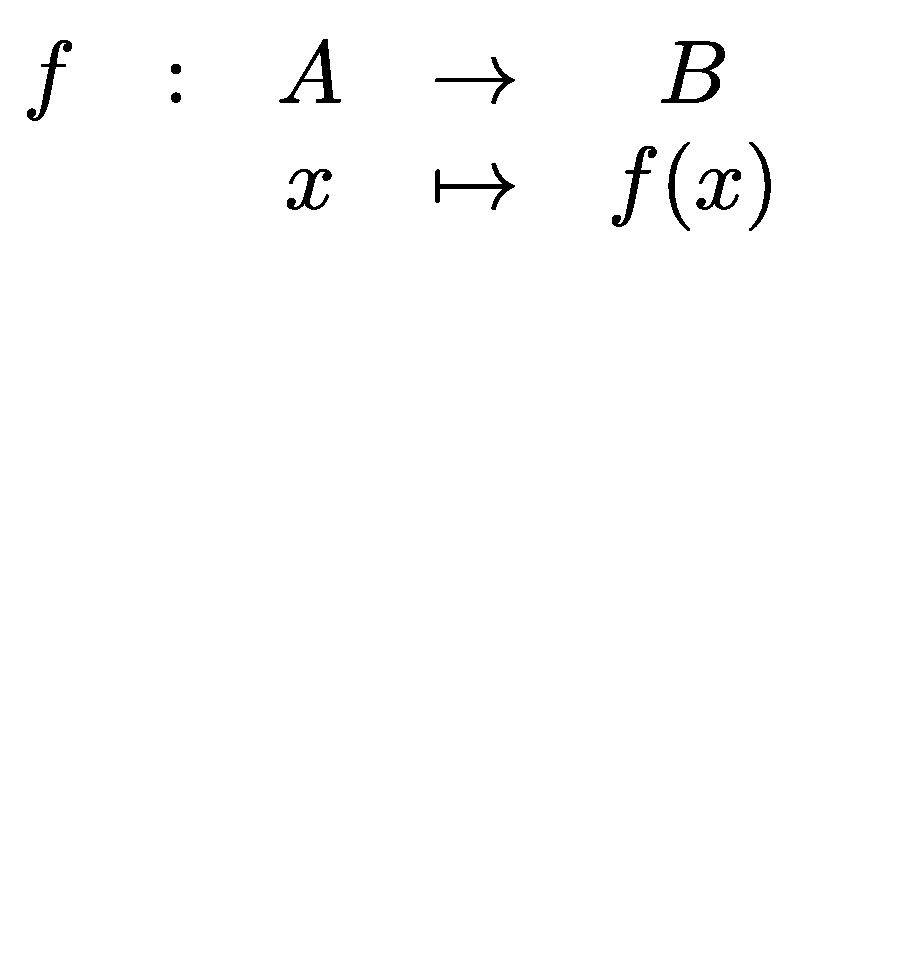
\includegraphics[width=0.5\linewidth]{images/fonctions_00.pdf}}
        \only<2>{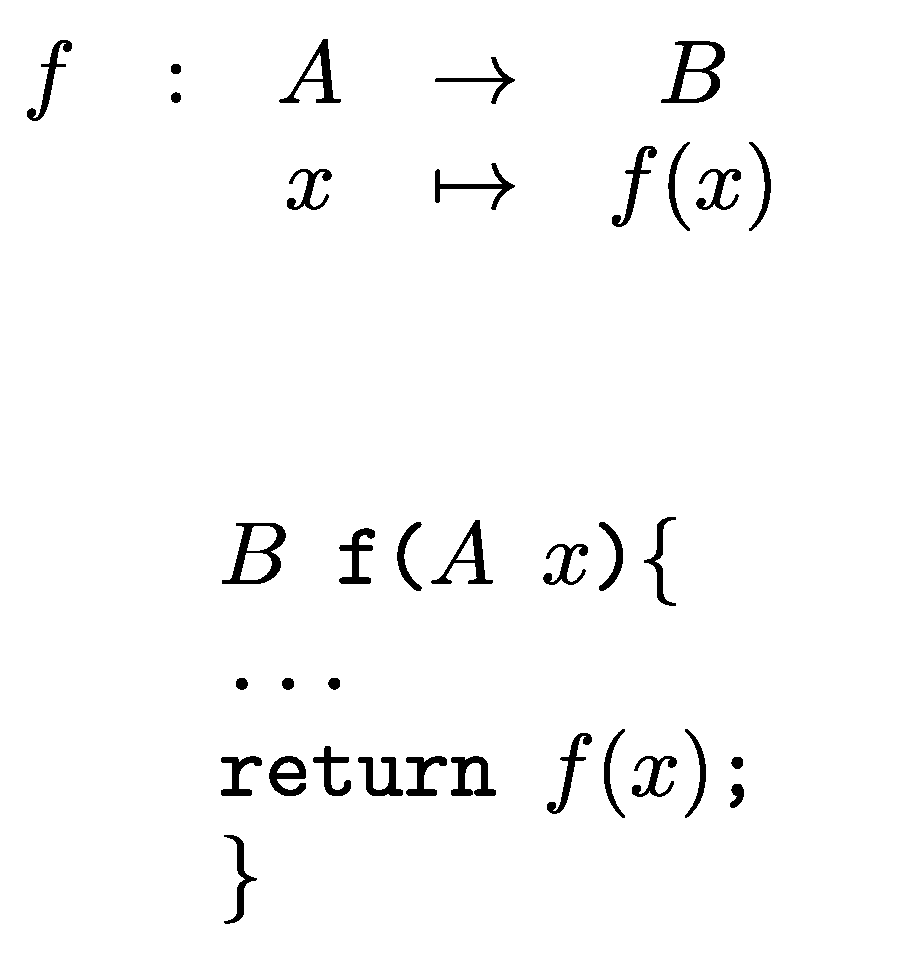
\includegraphics[width=0.5\linewidth]{images/fonctions_01.pdf}}
        \only<3>{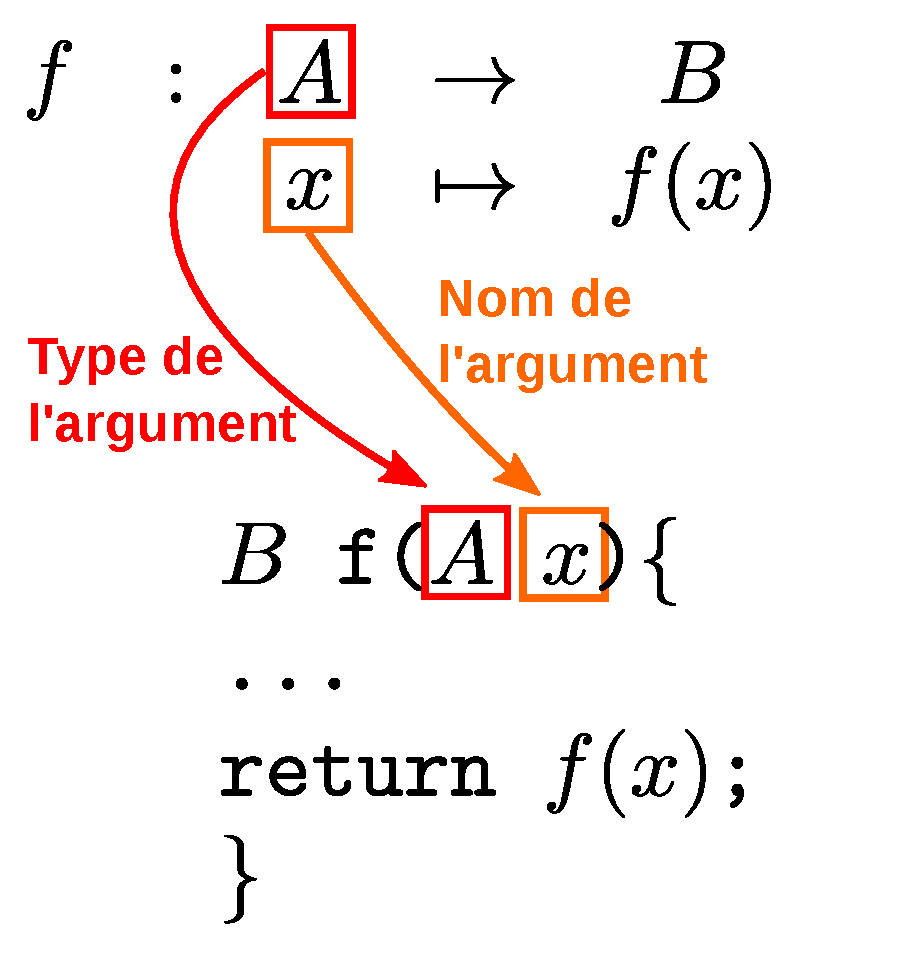
\includegraphics[width=0.5\linewidth]{images/fonctions_02.pdf}}
        \only<4>{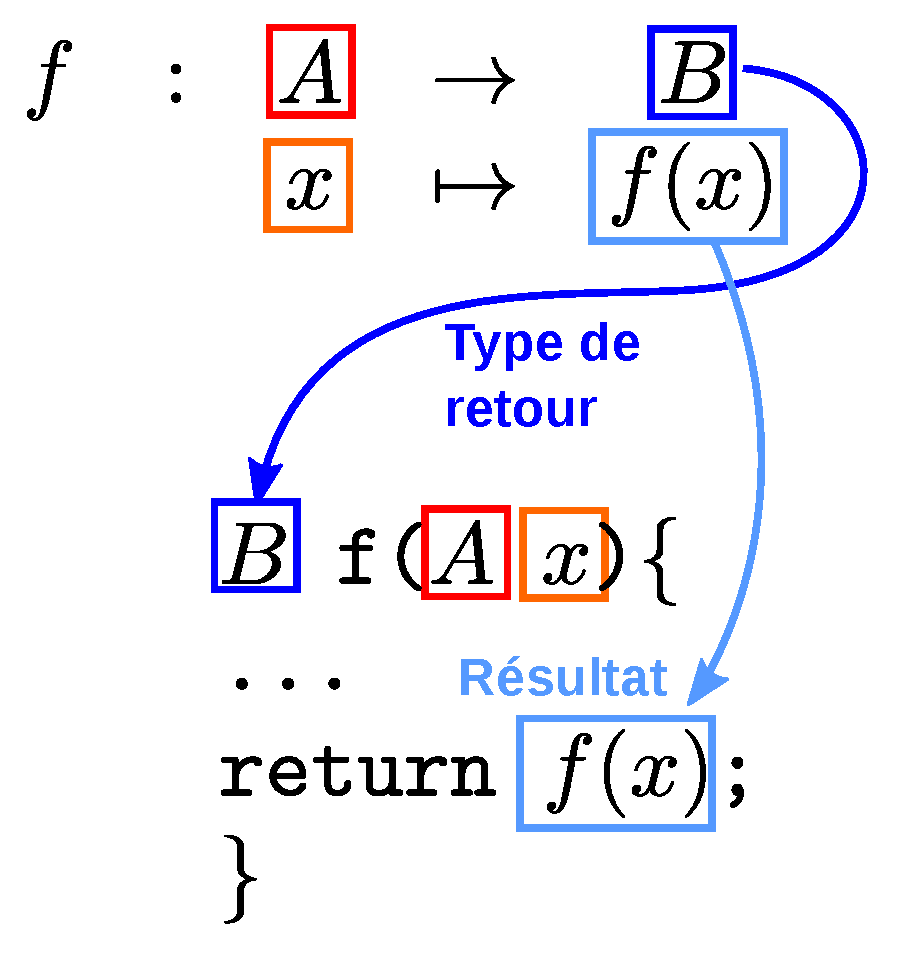
\includegraphics[width=0.5\linewidth]{images/fonctions_03.pdf}}
    \end{center}

\end{frame}

\begin{frame}[fragile]
\frametitle{Exemple}

\begin{block}{La fonction signe}
$$
\begin{array}{cccc}
signe: & \mathbb{R} & \to & \{-1,0,1\} \\
& x & \mapsto & \left\{
    \begin{split}
    -1 \: \text{si} \: x < 0\\
    1 \: \text{si}  \: x > 0\\
    0 \: \text{sinon}
    \end{split}
  \right.
\end{array}
$$
\end{block}
Deux manières d'écrire la même fonction.
\begin{minipage}{0.47\linewidth}
\begin{minted}{cpp}
int signe(double x){
  int s = 0;
	  
  if(x < 0)
    s = -1;
  if(x > 0)
    s = 1;
  return s;
}
\end{minted}
\end{minipage}
\hfill
\begin{minipage}{0.47\linewidth}
\begin{minted}{cpp}
int signe(double x){
    if(x < 0)
        return -1;
    if(x > 0)
        return 1;
    return 0;
}
\end{minted}
\end{minipage}
\end{frame}

\begin{frame}[fragile]
	\frametitle{Fonction sans retour}
	Pour des fonctions qui ne renvoient rien, on utilise le type de retour vide : \texttt{\textbf{void}}.

	Le retour vide : \texttt{\textbf{return;}} est optionnel.

	\begin{block}{Afficher}
	Afficher les coordonnées $(x,y,z)$ d'un vecteur :
		$$
		\begin{array}{cccc}
		affiche: & \mathbb{R}^3 & \to & \emptyset \\
		\end{array}
		$$
	\end{block}

	\begin{minted}{cpp}
void affiche(double x, double y, double z){
    cout << "(" << x << "," << y << "," << z << ")" << endl;
    return; // OPTIONNEL
}
void affiche(double x, double y, double z){
    cout << "(" << x << "," << y << "," << z << ")" << endl;
}
	\end{minted}
\end{frame}

\begin{frame}[fragile]
	\frametitle{Limitations}
	\begin{itemize}
	\item Il n'est pas possible de renvoyer plusieurs valeurs.
	\begin{minipage}{0.46\linewidth}
		\begin{minted}{python}
def f():
    a = 3
    b = 5
    return a, b # OK
		\end{minted}
	\end{minipage}
	\hfill
	\begin{minipage}{0.47\linewidth}
		\begin{minted}{cpp}
int f(){
   int a = 3, b = 5;
   return a, b; // ERREUR
}
		\end{minted}
	\end{minipage}
	\item On ne peut pas modifier les arguments (ils sont copiés).
	\begin{minipage}{0.46\linewidth}
			\begin{minted}{cpp}
void switch_1(double a,
              double b){
    // Échange a et b
    double c = b;
    b = a;
    a = c;
}
			\end{minted}
		\end{minipage}
		\hfill
		\begin{minipage}{0.51\linewidth}
			\begin{minted}{cpp}
int main(){
    double x = 5, y = 7;
    switch_1(x,y);
    cout << x << ", " << y;
    // Affiche "5, 7"
}
			\end{minted}
		\end{minipage}
	\end{itemize}
\end{frame}

\begin{frame}
	\frametitle{Le passage par référence}

  Ces problèmes sont dus à la copie qui est réalisée lorsque l'on entre dans une fonction.

	Le passage par référence est une solution aux problèmes précédents. Il autorise la modification de l'argument concerné en le préfixant dans la signature de la fonction par \texttt{\&}.

	\begin{block}{Syntaxe}
	\texttt{type f(type1 {\huge\textbf{\&}} arg1, type2 {\huge\textbf{\&}} arg2, type3 arg3 ...)\{...\}}
	\end{block}
\end{frame}

\begin{frame}[fragile]
	\frametitle{Passage par référence : exemples}
	\begin{itemize}
	\item "Renvoyer" deux ou plus valeurs (modifier les arguments)
	\begin{minipage}{0.49\linewidth}
		\begin{minted}{cpp}
void f(int & a, int & b){
   a = 3;
   b = 5;
}
		\end{minted}
	\end{minipage}
	\hfill
	\begin{minipage}{0.47\linewidth}
		\begin{minted}{cpp}
int main(){
   int x = 0, y = 0;
   f(x, y);
   cout << x << ", " << y;
   // Affiche "3, 5"
}
		\end{minted}
	\end{minipage}
	\item Modifier les arguments

	\begin{minipage}{0.49\linewidth}
			\begin{minted}{cpp}
void switch_2(double & a,
              double & b){
    // Échange a et b
    double c = b;
    b = a;
    a = c;
}
			\end{minted}
		\end{minipage}
		\hfill
		\begin{minipage}{0.47\linewidth}
			\begin{minted}{cpp}
int main(){
    double x = 5, y = 7;
    switch_2(x,y);
    cout << x << ", " << y;
    // affiche 7, 5
}
			\end{minted}
		\end{minipage}
	\end{itemize}
\end{frame}

\begin{frame}
\frametitle{Passage par référence : zoom sur la mémoire 1}
Fonctionnement de la fonction \texttt{switch\_1}
\centering
\only<1>{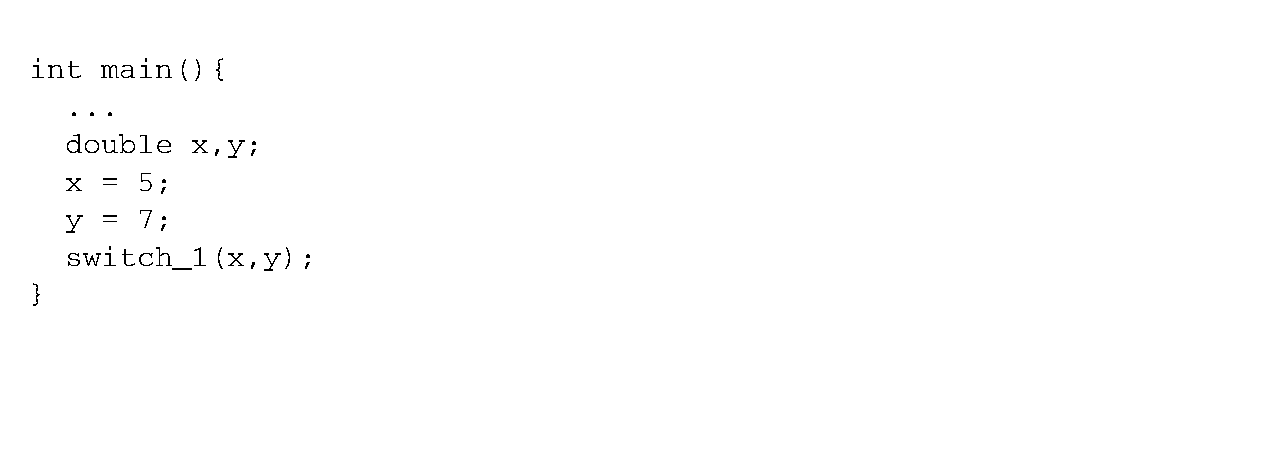
\includegraphics[width=\linewidth]{images/switch_1_00.pdf}}
\only<2>{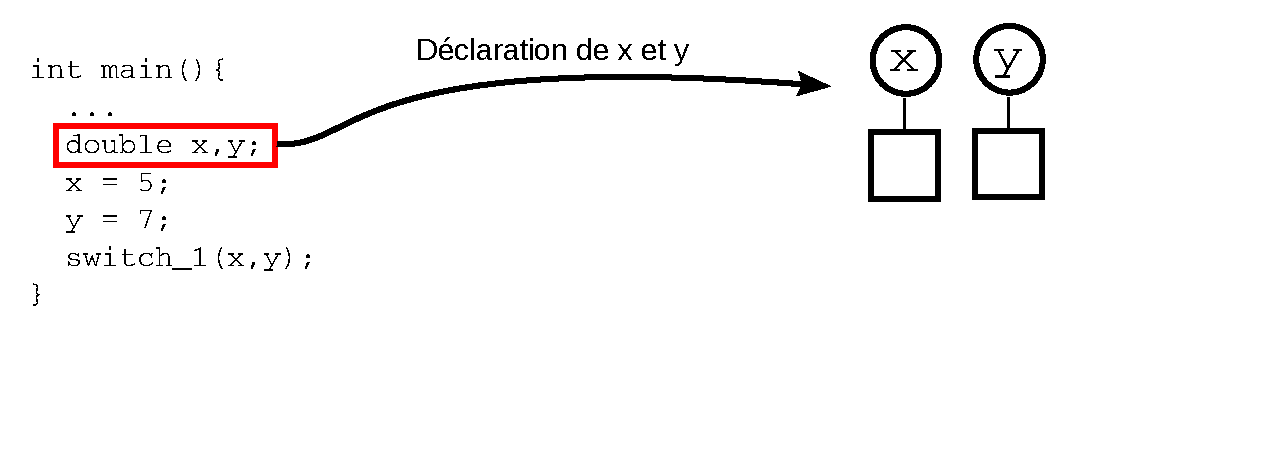
\includegraphics[width=\linewidth]{images/switch_1_01.pdf}}
\only<3>{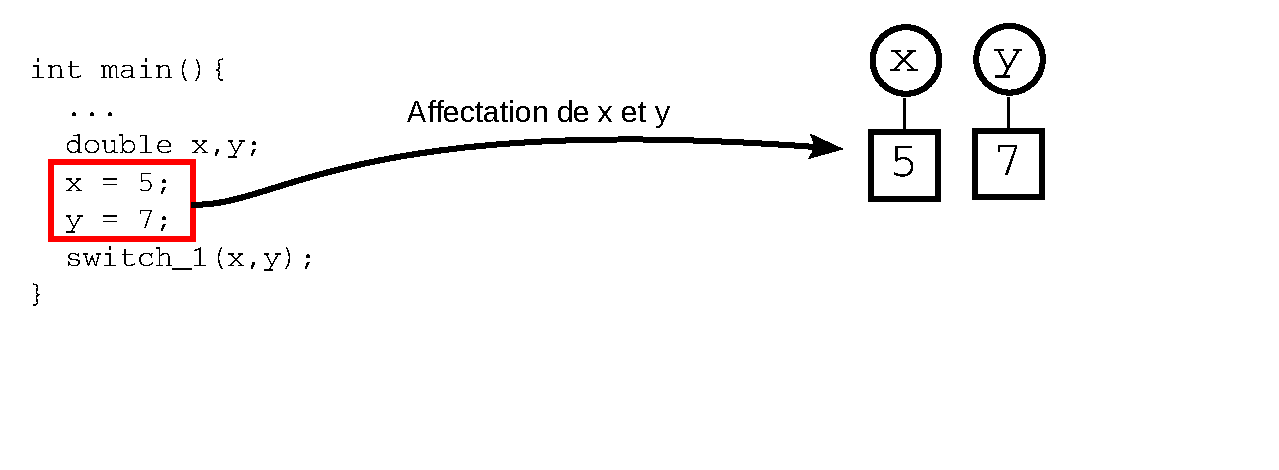
\includegraphics[width=\linewidth]{images/switch_1_02.pdf}}
\only<4>{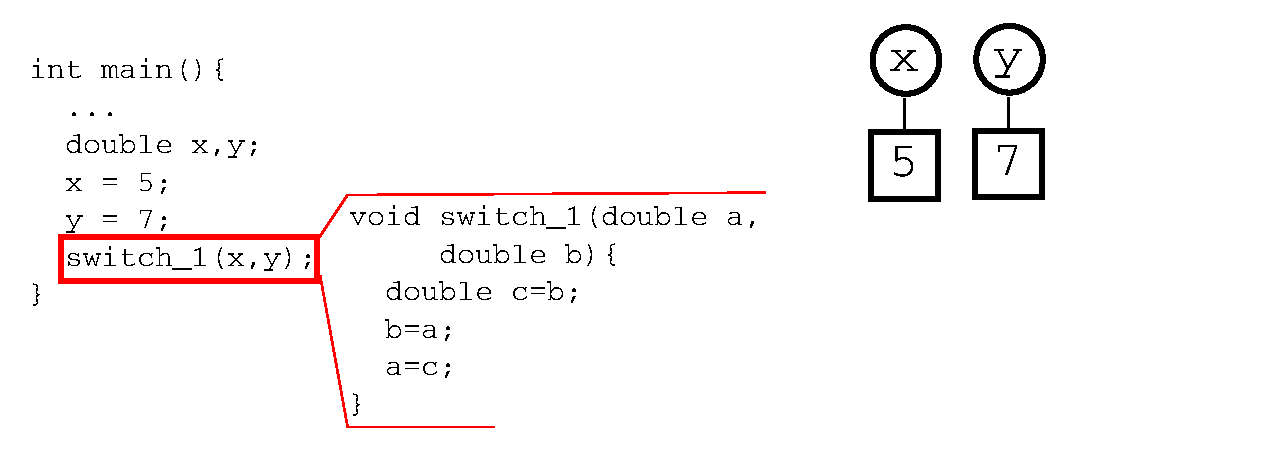
\includegraphics[width=\linewidth]{images/switch_1_03.pdf}}
\only<5>{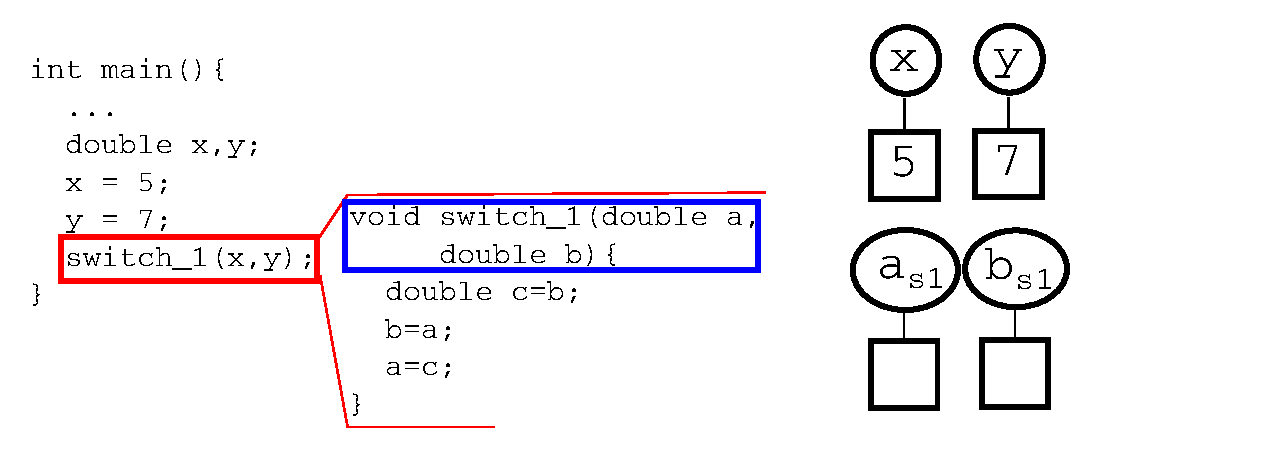
\includegraphics[width=\linewidth]{images/switch_1_04.pdf}}
\only<6>{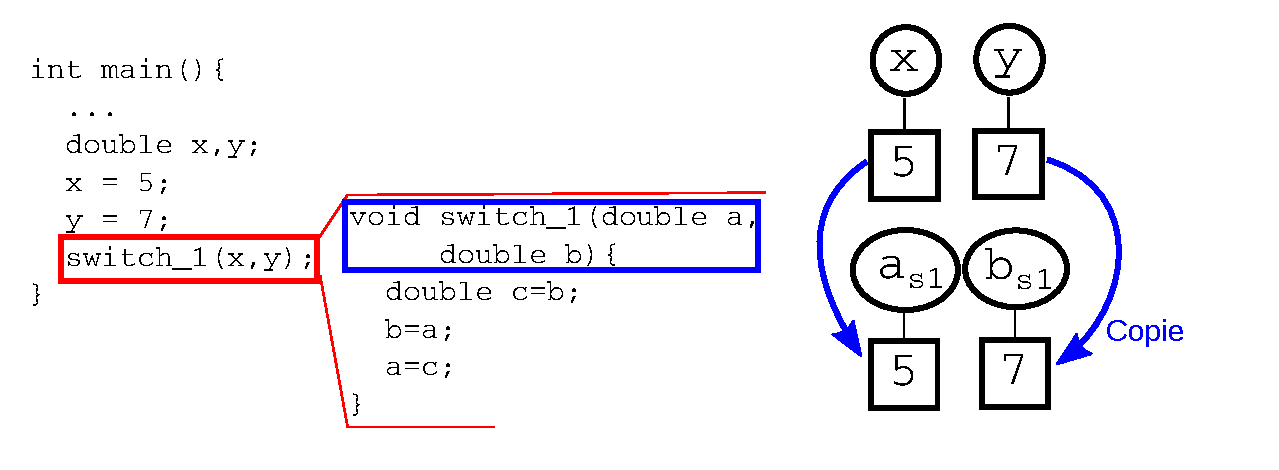
\includegraphics[width=\linewidth]{images/switch_1_05.pdf}}
\only<7>{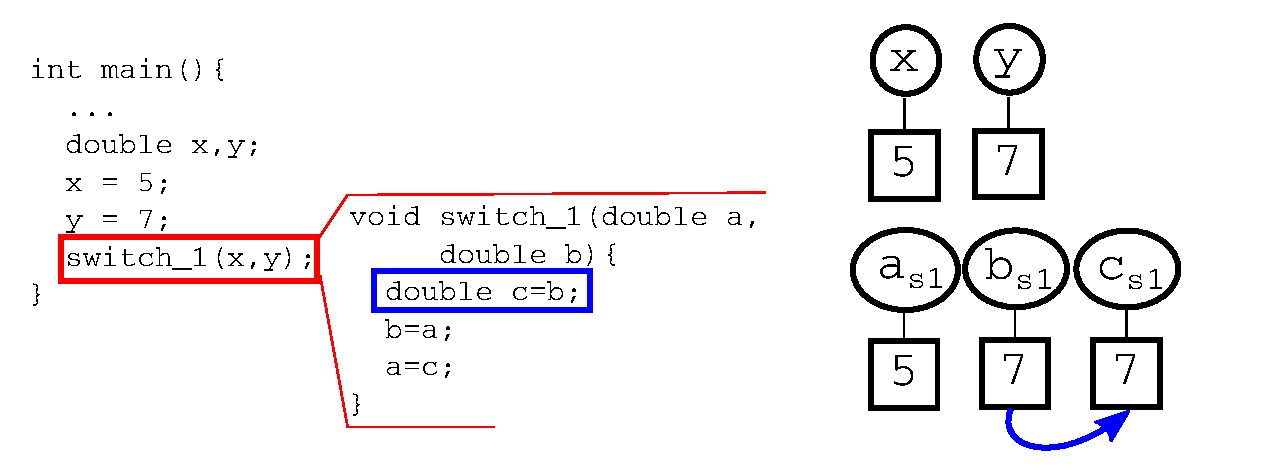
\includegraphics[width=\linewidth]{images/switch_1_06.pdf}}
\only<8>{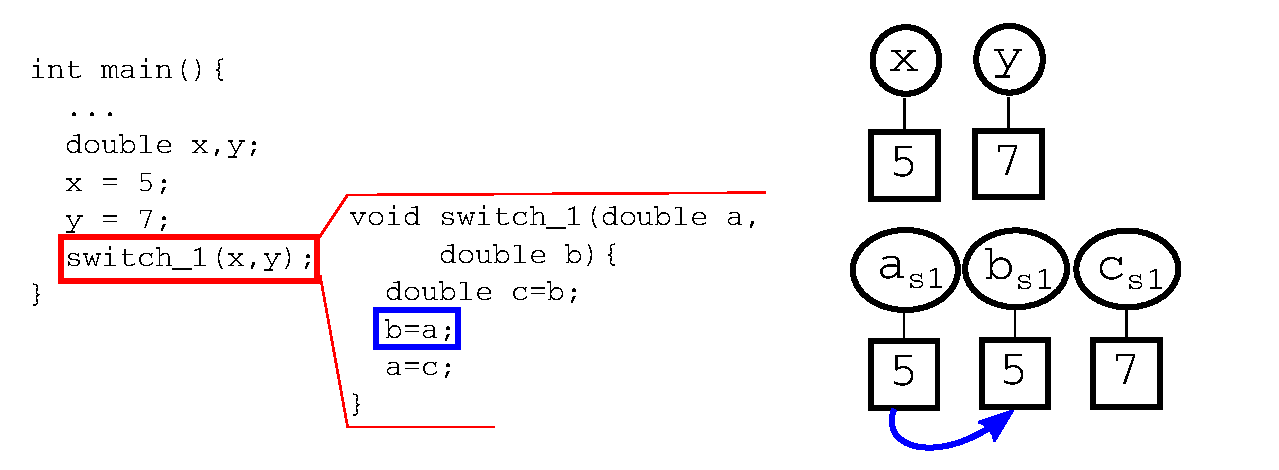
\includegraphics[width=\linewidth]{images/switch_1_07.pdf}}
\only<9>{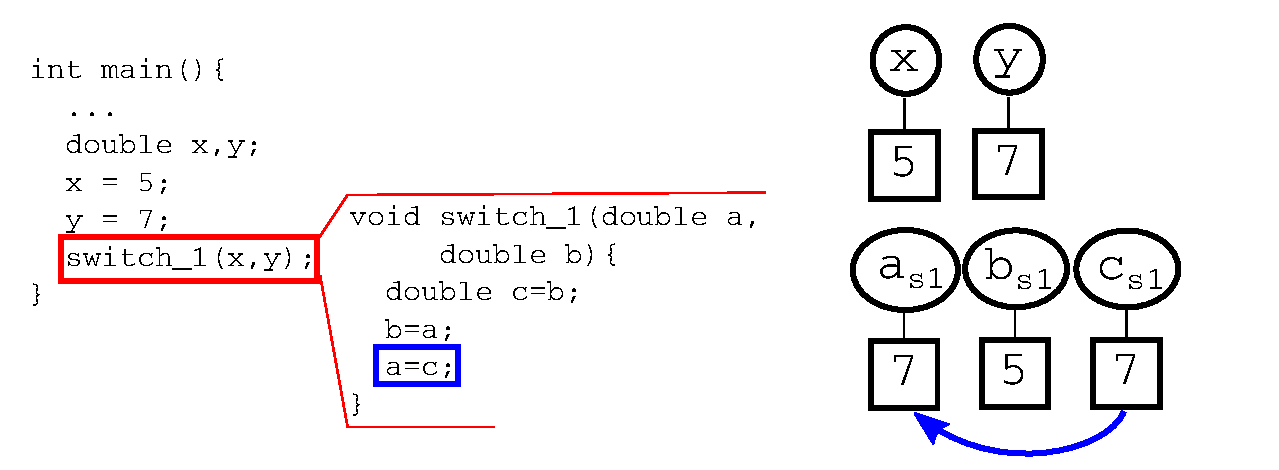
\includegraphics[width=\linewidth]{images/switch_1_08.pdf}}
\only<10>{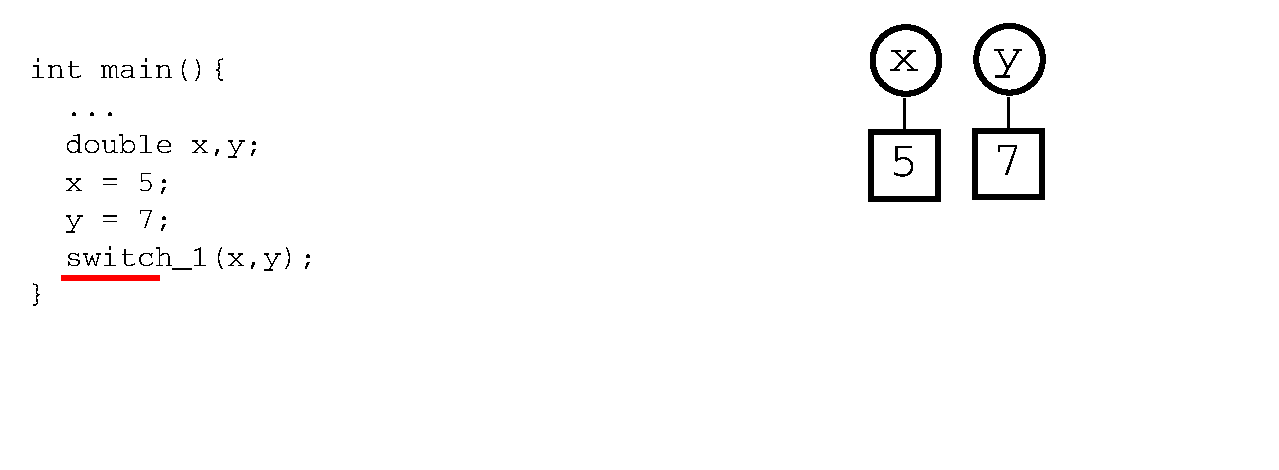
\includegraphics[width=\linewidth]{images/switch_1_09.pdf}}
\end{frame}


\begin{frame}
\frametitle{Passage par référence : zoom sur la mémoire 2}
Fonctionnement de la fonction \texttt{switch\_2}
\centering
\only<1>{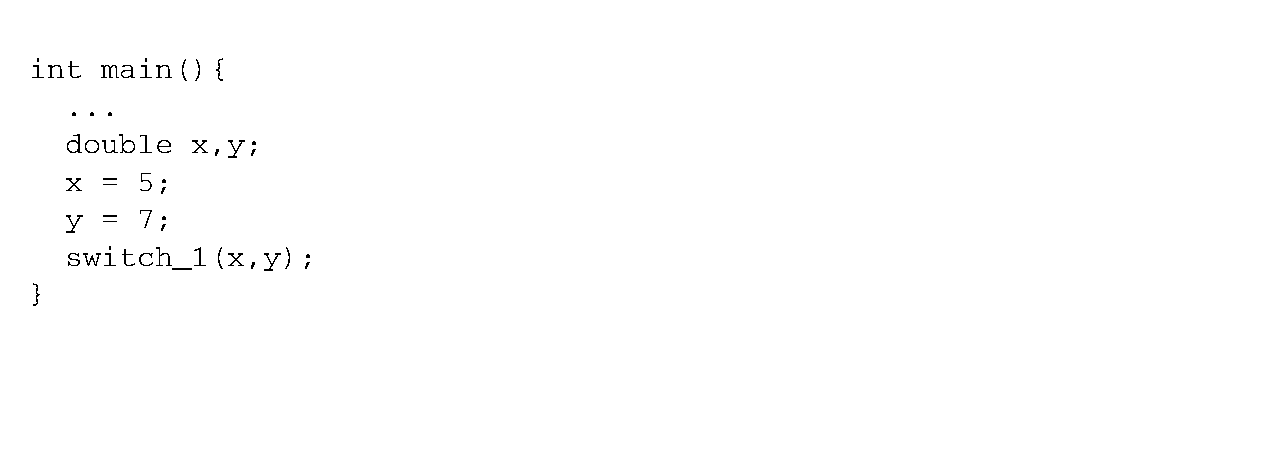
\includegraphics[width=\linewidth]{images/switch_1_00.pdf}}
\only<2>{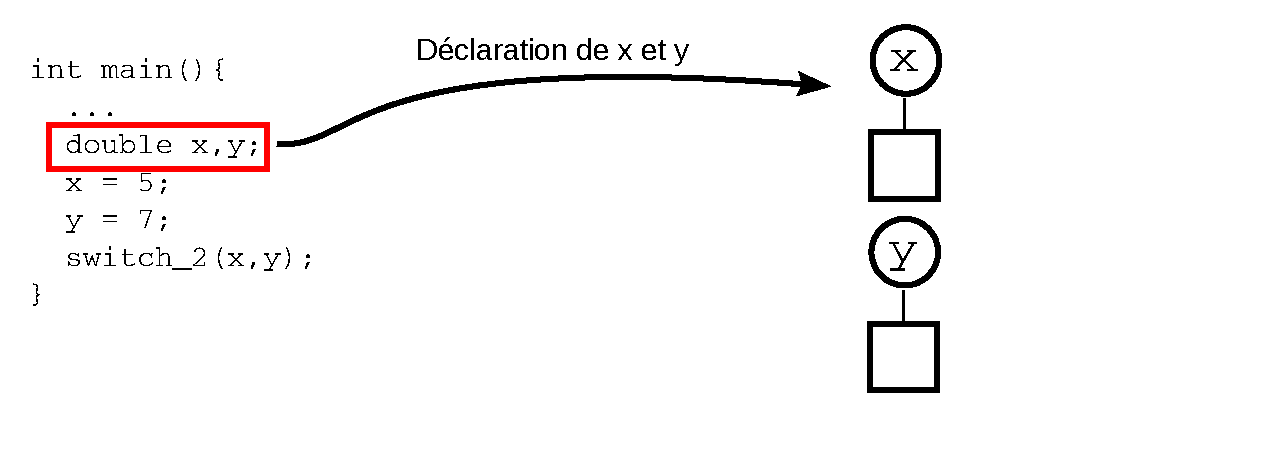
\includegraphics[width=\linewidth]{images/switch_2_00.pdf}}
\only<3>{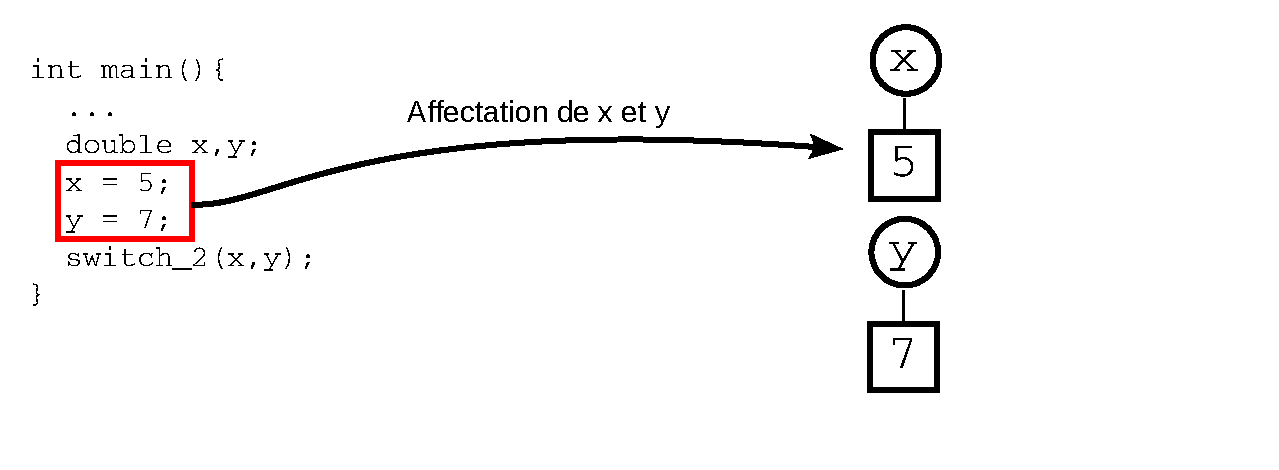
\includegraphics[width=\linewidth]{images/switch_2_01.pdf}}
\only<4>{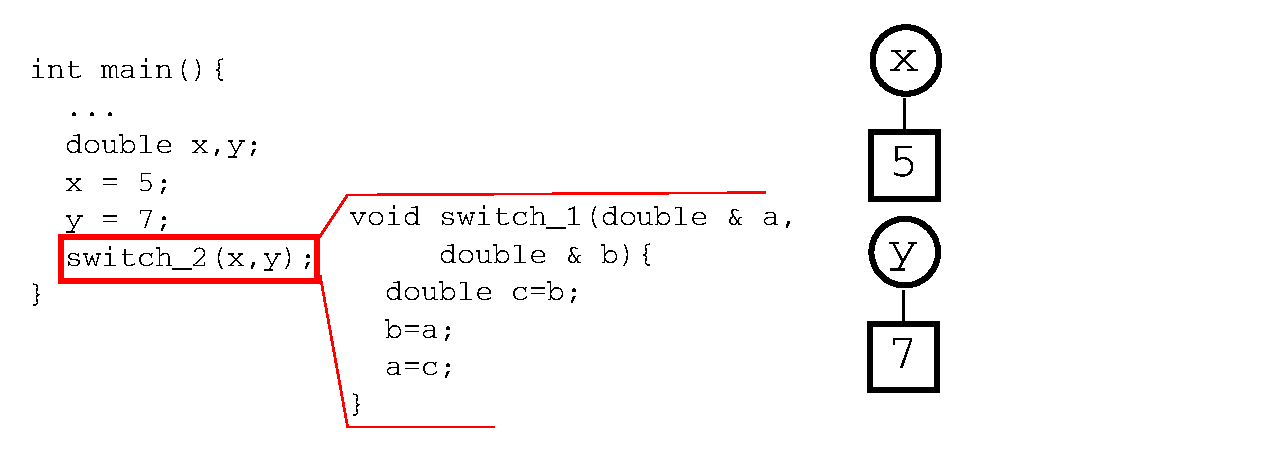
\includegraphics[width=\linewidth]{images/switch_2_02.pdf}}
\only<5>{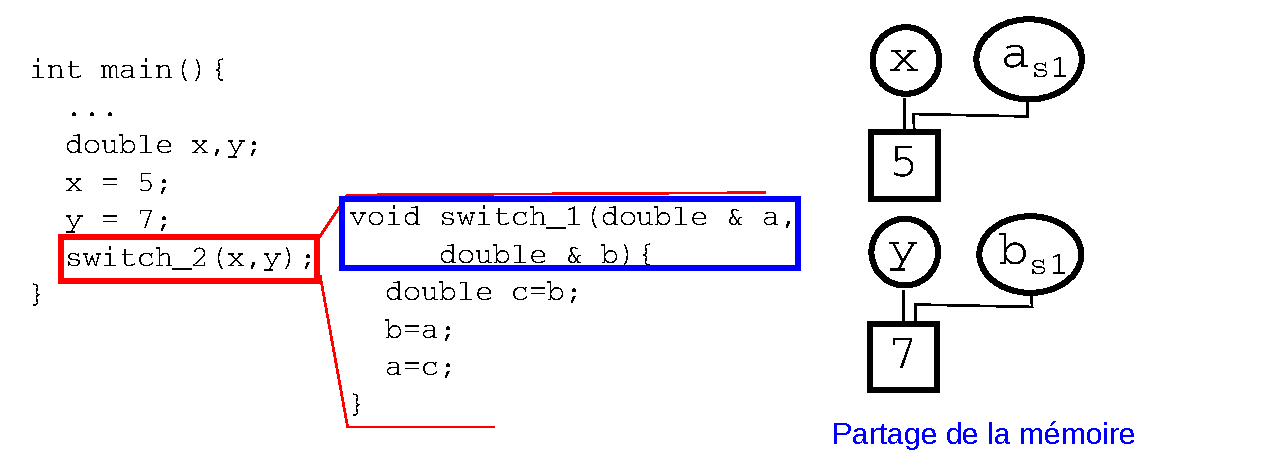
\includegraphics[width=\linewidth]{images/switch_2_03.pdf}}
\only<6>{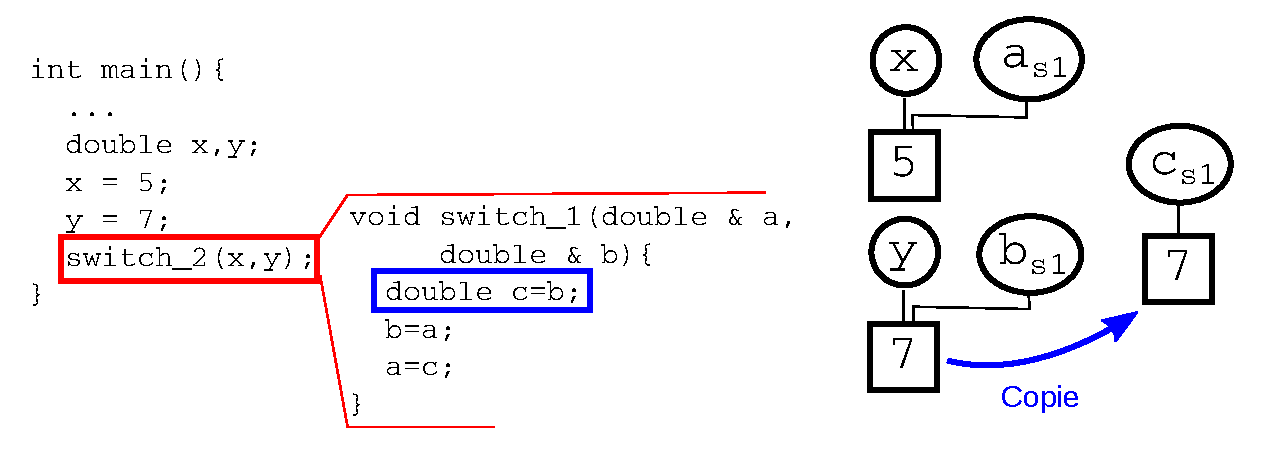
\includegraphics[width=\linewidth]{images/switch_2_04.pdf}}
\only<7>{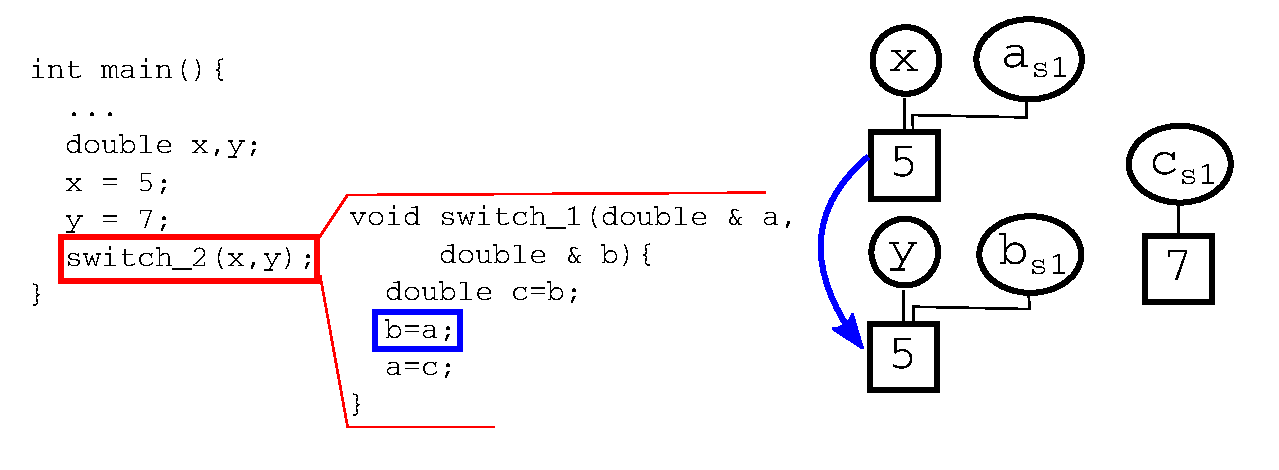
\includegraphics[width=\linewidth]{images/switch_2_05.pdf}}
\only<8>{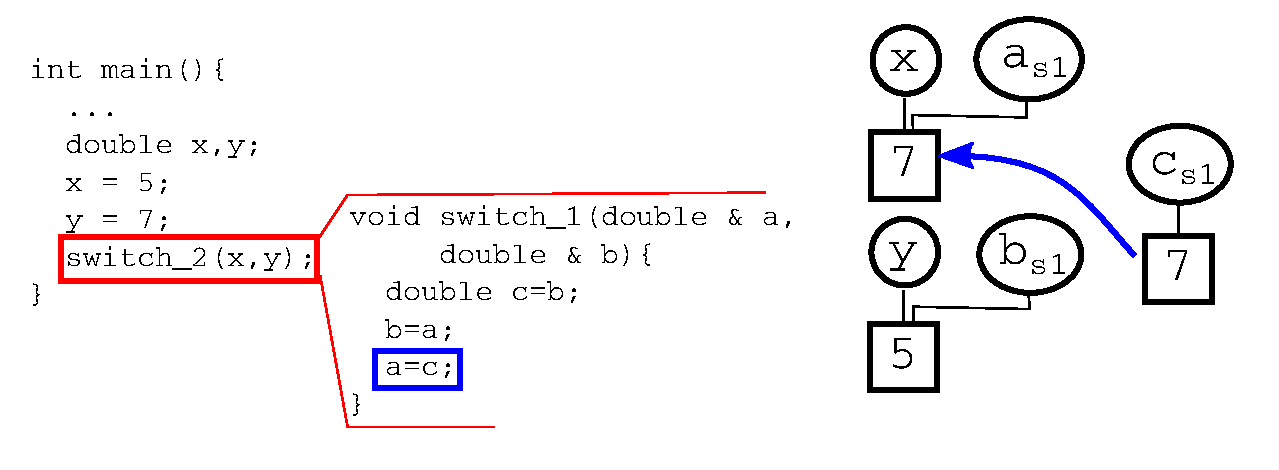
\includegraphics[width=\linewidth]{images/switch_2_06.pdf}}
\only<9>{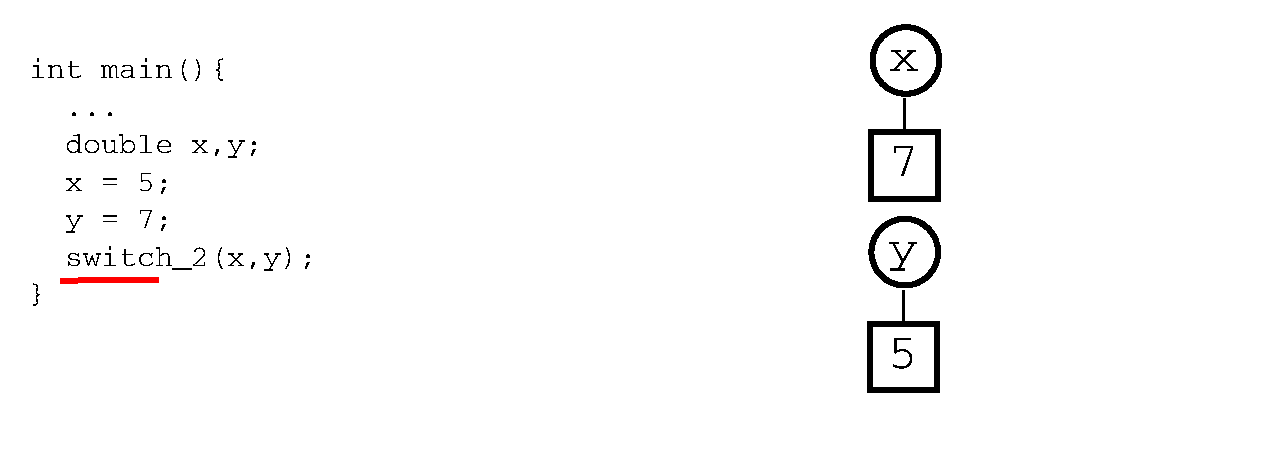
\includegraphics[width=\linewidth]{images/switch_2_07.pdf}}
\end{frame}

\begin{frame}[fragile]{Exemples}
\setbeamercovered{} 
\onslide<1->
\begin{minted}{cpp}
int f(double a, int &b){
  a = 2.5;
  b = 1;
  return a/b;
}
double a = 3.14;
int b = 2;
int c = f(a,b);
// Que valent a, b et c ?
\end{minted}
\vspace*{-1em}
\onslide<2->
\begin{minted}{cpp}
// a = 3.14 (pas modifié), b = 1 (référence), c = 2 car c'est un int !
\end{minted}

\vspace*{-1em}
\onslide<3->
\begin{minted}{cpp}
double g(double &a, double &b){
  return (a + b)/2;
}
double a = 9, b = 0;
double c = g(a,b); 
// Que valent a, b et c ?
\end{minted}
\vspace*{-1em}
\onslide<4-> 
\begin{minted}{cpp}
// a=9 et b=0 sont passés par référence mais non modifiés, c=4.5
\end{minted}
\end{frame}


\begin{frame}[fragile]
	\frametitle{Surcharge}
	Il est possible de donner le même nom à deux fonctions (ou plus) à condition que les types ou le nombre des arguments de celles-ci soient différents. Autrement, deux fonctions peuvent avoir le même nom si leurs signatures diffèrent.
	\vfill
	\begin{minipage}{0.47\linewidth}
	\begin{minted}{cpp}
int f(int v1, int v2){
    return v1 + v2;
}

double f(int v1, int v2){
    return 0.5;
}

// ERREUR !!!
// Même nom +
// arguments identiques
	\end{minted}
	\end{minipage}
	\hfill
	\begin{minipage}{0.47\linewidth}
	\begin{minted}{cpp}
int f(int v1, int v2){
    return v1 + v2;
}

double f(int v1, int v2, int v3){
    return 0.5;
}

// OK
// Même nom mais
// arguments différents
	\end{minted}
	\end{minipage}

\end{frame}

\begin{frame}[fragile]
	\frametitle{Portée, déclaration}

	\begin{block}{Appel de fonction}
		Comme pour les variables on ne peut utilisée une fonction que si elle a été déclarée préalablement.
	\end{block}
	\vfill

	\begin{minipage}{0.47\linewidth}

	\begin{minted}{cpp}
void f(){
    g(3);
    // ERREUR g est inconnue
}

void g(int i){
    ...
}
	\end{minted}
	\end{minipage}
	\hfill
	\begin{minipage}{0.47\linewidth}
	\begin{minted}{cpp}
void g(int i){
   ...
}

void f(){
    g(3); //OK
}
	\end{minted}
	\end{minipage}
\end{frame}

\begin{frame}[fragile]
	\frametitle{Portée, déclaration}

	\begin{minipage}{0.47\linewidth}
		\begin{minted}{cpp}
void f(){
    g(3);
    // ERREUR g est inconnue
}

void g(int i){
    f();
}
		\end{minted}
	\end{minipage}
	\hfill
	\begin{minipage}{0.47\linewidth}

		\begin{minted}{cpp}
void g(int i); // Déclaration

void f(){
    g(3); // OK

// Définition
void g(int i){
    ...
}
		\end{minted}
	\end{minipage}
\end{frame}

\begin{frame}[fragile]
	\frametitle{Variables locales et globales}

	\begin{block}{Variables globales}
		Les variables globales sont déclarées en dehors des fonctions.
		Elles sont accessibles à l'ensemble du programme.
	\end{block}

	\begin{minipage}{0.47\linewidth}
		\begin{minted}{cpp}
void f(){
    ...
    int i1 = 3;
    ...
}

void g(int i){
    cout << i1 << endl;
    /* ERREUR i1 inconnu
       i1 est une variable
       de f */
}
		\end{minted}
	\end{minipage}
	\hfill
	\begin{minipage}{0.47\linewidth}

		\begin{minted}{cpp}
int i1; // variable globale

void f(){
    ...
    i1 = 3;
    ...
}

void g(int i){
    cout << i1 << endl;
    /* OK i1 est une variable
       globale */
}
		\end{minted}
	\end{minipage}

\end{frame}


\begin{frame}[fragile]
	\frametitle{Variables locales et globales}

\begin{alertblock}{Attention}
	L'usage des variables globales est à limiter au maximum :
	\begin{itemize}
		\item La communication entre les fonctions est source de bugs.
		\item Elles rendent les fonctions difficilement réutilisables.
	\end{itemize}
\end{alertblock}

\begin{block}{Usage}
	Les variables globales sont des constantes générales.
\end{block}

\begin{minted}{cpp}
const int width = 800; // constante non modifiable
const int height = 600;

int main(){
    ...
    openWindow(width, height);
    ...
    height = 5; // ERREUR : height est une constante
}
\end{minted}

\end{frame}


\section{TP}

\begin{frame}{Organisation des TPs}
    \begin{itemize}
        \item En salle informatique de 9h45 à 11h15.
        \item Par groupe de 2
        \item Sur machine de l'école ou machine perso
        \item OS au choix
            \begin{itemize}
                \item Machine perso : Linux, Windows, OSX
                \item École : Windows, Linux
            \end{itemize}
        \item IDE au choix (QtCreator recommandé)
        \item \alert<+>{À rendre sous forme d'archive \texttt{.zip} sur \textbf{Educnet} avant le \textbf{26/09}}
        \item \alert<+>{\textbf{Exercice individuel} à rendre pour le \textbf{3/10}}
    \end{itemize}
\end{frame}

\begin{frame}{TP de la semaine}

	\begin{block}{Sujet}
        \begin{itemize}
            \item Utilisation du débogueur
            \item Prise en main de la bibliothèque Imagine++
            \item Programmation d'un mini-jeu de tennis
        \end{itemize}
	\end{block}
  \begin{center}
    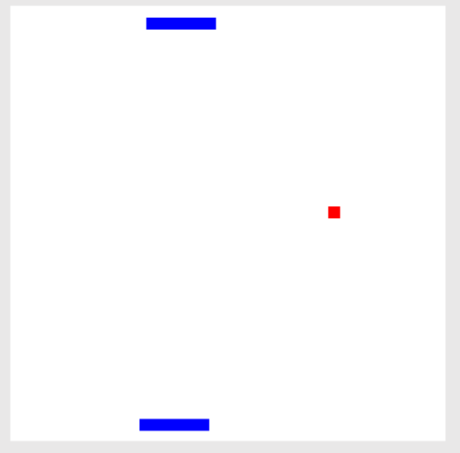
\includegraphics[width=0.38\textwidth]{images/tennis}
  \end{center}
\end{frame}

\end{document}
